% 서울대학교 전기·정보공학부 학사 학위논문 템플릿
% 논문 작성 지침에 일부 부합하지 않는 부분이 있을 수 있습니다.

\documentclass[10pt,a4paper]{report}
\usepackage{amssymb, amsmath, mathtools} % 수학
\usepackage{siunitx} % SI단위
\usepackage{graphicx} % 그림
\usepackage{booktabs} % 표
\usepackage{indentfirst} % 첫 문장 들여쓰기

\usepackage[style=ieee]{biblatex} % IEEE형식 참고문헌
\addbibresource{citations.bib}

\usepackage{tikz} % 그림 그리기
\usetikzlibrary{positioning}

\usepackage[hangul]{kotex} % 한글
\usepackage[HWP]{dhucs-interword} % 아래아한글 자간
\usehangulfontspec{default}

%\usepackage[list=off]{bicaption} % 이중 캡션
%\captionsetup[table][bi-second]{name=Table}
%\captionsetup[figure][bi-second]{name=Figure}
%\usepackage{subcaption}

\def\papertitle{Numerical and Analytical Analysis of Squeezed Vacuum States of Light by Means of Wigner Functions} % 제목
\def\paperdate{2023년 8월} % 발간(연월
\def\paperauthor{이준협} % 저자
\def\paperauthorspaced{이 준 협}
\def\paperadvisor{정윤찬} % 지도교수
\def\paperkeywords{압축 광원, 위상 공간 분석, 위그너 함수} % 국문 키워드
\def\paperenglishkeywords{squeezed light, phase space method, Wigner function} % 영문 키워드

\usepackage[pdfauthor={\paperauthor},
            pdftitle={공학 학사 학위논문},
            pdfsubject={\papertitle},
            pdfkeywords={\paperkeywords, \paperenglishkeywords},
            ]{hyperref} % PDF

% 여백
\addtolength{\hoffset}{-1in}
\addtolength{\voffset}{-1in}
\setlength{\topmargin}{30mm}
\setlength{\headheight}{0mm}
\setlength{\headsep}{0mm}
\setlength{\marginparwidth}{0mm}
\setlength{\marginparsep}{0mm}
\setlength{\oddsidemargin}{25mm}
\setlength{\textwidth}{160mm}
\setlength{\textheight}{227mm}
\setlength{\footskip}{20mm}
\linespread{1.6} % double spacing 줄간격

% \chapter*도 목차에 추가
\makeatletter
\def\@makeschapterhead#1{%
  \addcontentsline{toc}{chapter}{#1}%
  {\centering\parindent \z@
    \normalfont
    \interlinepenalty\@M
    \Huge \bfseries  #1\par\nobreak
    \vskip 40\p@
  }}
\makeatother

\pagenumbering{alph} % 임시 알파벳 페이지 번호

% rotated wigner function
\newcommand*{\wigner}{
W(\omega z, \omega^{-1}z^{*};t)}

% bra-ket
\newcommand*\bra[1]{\langle{#1}|}
\newcommand*\ket[1]{|{#1}\rangle}

\usepackage{titlesec}
\titleformat{\chapter}[display]
{\normalfont\huge\bfseries}
{Chapter \thechapter}{20pt}{\Huge}

\begin{document}
\renewcommand{\abstractname}{초~록}
\renewcommand{\figurename}{Figure}
\renewcommand{\contentsname}{Contents}
\renewcommand{\listtablename}{List of Tables}
\renewcommand{\listfigurename}{List of Figures}

\thispagestyle{empty} % 외표지
\begin{center}
    \fontsize{16pt}{19pt}\selectfont
    공학 학사 학위논문 \\
    \vspace{2cm}
    \fontsize{21pt}{25pt}\selectfont
    \papertitle \\
    \vfill
    \fontsize{16pt}{19pt}\selectfont
    \paperdate \\
    \vspace{4cm}
    서울대학교 공과대학 \\
    \vspace{1cm}
    전기·정보공학부 \\
    \vspace{1cm}
    \paperauthorspaced
\end{center}
\newpage

\thispagestyle{empty} % 인준지
\begin{center}
    \fontsize{21pt}{25pt}\selectfont
    \papertitle \\
    \vspace{1cm}
    \fontsize{16pt}{19pt}\selectfont
    지도교수 \paperadvisor \\
    \vspace{1cm}
    이 논문을 공학 학사학위 논문으로 제출함. \\
    \vfill
    서울대학교 공과대학 \\
    \vspace{1cm}
    전기·정보공학부 \\
    \paperauthorspaced \\
    \vspace{1cm}
    \paperauthor의 학사 학위 논문을 인준함. \\
    \vspace{1cm}
    2023년 ~~~~~~월 ~~~~~~일 \\
    \vspace{1cm}
    지도교수 ~~~~~~~~~~~~~~~~~~~~~~~~~~~~~~~~(인)
\end{center}
\newpage

\pagenumbering{roman} % 로마 숫자 페이지 번호
\chapter*{Abstract}

This thesis aims to illustrate the effectiveness of the phase space method by analyzing second- and higher-order squeezing of light using the Wigner quasiprobability distribution. Using numerical methods, we first illustrate the quasiprobability distribution of the photon under squeezing, which gives an intuitive picture of how the uncertainty is squeezed. Furthermore, by applying the phase space method, we prove that second-order squeezing applies for arbitrary initial distributions, and that higher order squeezing preserves the initial symmetry of the vacuum state of light.

\vfill
Keywords: \paperenglishkeywords

{ % 목차
\renewcommand\baselinestretch{1.3}
\tableofcontents
%\listoftables
\listoffigures
}

\chapter{Introduction}\label{chap:introduction}
\pagenumbering{arabic}
Quantum mechanics tells us that the fundamental limitation of measurements is given by the uncertainty product $\Delta x\Delta p\ge\hbar/2$.
Since all phenomena are inherently quantum, all generalized position and momentum variables cannot be measured with arbitrary precision.
This is also true for the case of EM waves. Consider the TEM field given by:
\begin{equation}
  \vec{E}_{\mathbf{k},\lambda}(\vec{r},t)=\vec{e}_{\mathbf{k},\lambda}(p\cos{(\mathbf{k}\cdot\vec{r}-ckt)}+q\sin{(\mathbf{k}\cdot\vec{r}-ckt)})
\end{equation}
Here the coefficients $q$ and $p$ are the generalized position and momentum variables, and the uncertainty product satisfies
\begin{equation}
  \Delta p\Delta q \ge \frac{\hbar ck}{2\varepsilon_{0}L^{3}}
\end{equation}
when $[0,L]^{3}$ is the cavity we are interested in(in real life, this cavity is carefully set up in experiments as to reduce interference from the environment).

If we rewrite $p\cos{\theta(t)}+q\sin{\theta(t)}=A\sin{(\theta(t)+\phi)}$, we can conclude that the phase and amplitude cannot be both measured with arbitrary precision.
However, we may consider methods to suppress the uncertainty of $\Delta q$ at the cost of a bigger $\Delta p$.
That is, we want to ``squeeze'' the uncertainty in one direction, while preserving the minimum uncertainty product.

Especially, quantum mechanics tells us that there is noise in \textit{vacuum}, due to the nonzero energy level in vacuum.
This noise is called ``shot noise'', and squeezing the ``vacuum states of light'' enables measurements at sub shot-noise levels.
According to Lawrie et al., this has practical implications in ``high energy physics, biochemistry, and scanning probe microscopy''\cite{qsensing}.

This thesis explains a method called the ``phase space method'', which converts equations concerning quantum mechanical operators to differential equations concerning ``quasiprobability distributions''.
Among the various quasiprobability distributions proposed, we use the Wigner function to analyze second- and higher-order squeezing.
Since phase space methods allow reasoning in terms of the probability distribution directly, we claim that this method allows one to develop intuition on why quantum systems behave the way they do.
Concretely, the phase space method straightforwardly explains why the probability distribution of higher order squeezing display ``rotational symmetry'' in vacuum.

\section{Quantization of the Maxwell Equations}
Before delving into the equations that describe squeezing, we first need to reduce the Maxwell equations into the one-dimensional simple harmonic oscillator(SHO).
The derivations are from \cite{loudon}.

We start with the description of Maxwell equations in terms of the vector potential $\vec{A}$ and scalar potential $\phi$.
Under the Coulomb gauge,
$\vec{E}=-\nabla\phi-\partial_{t}\vec{A}$ and $\vec{B}=\nabla\times\vec{A}$, then the Maxwell equations reduce to:

\begin{equation}
  (\nabla^{2}-\varepsilon_{0}\mu_{0}\partial_{t}^{2})\vec{A}=-\mu_{0}\vec{J}-\nabla(\partial_{t}\phi)\qquad
  \nabla^{2}\phi=-\rho
\end{equation}

It turns out that interpreting the vector potential for each mode and polarization as the annihilation operator $\hat{a}$ gives the energy of the electric field perfectly.
\begin{align}
  \vec{A}=\vec{\alpha}e^{i(\mathbf{k}\cdot\vec{r}-\omega_{\mathbf{k}}t)}\Rightarrow\omega_{\mathbf{k}}^{2}=c^{2}k^{2},\vec{\alpha}\cdot\mathbf{k}=0\qquad
  \text{Harmonic Oscillator}                                                                                                                                                             \\
  \vec{A}_{\mathbf{k},\lambda}=\vec{e}_{\mathbf{k},\lambda}\Re\{\alpha_{\mathbf{k},\lambda}e^{i(\mathbf{k}\cdot\vec{r}-ckt)}\}(\mathbf{k}=2\pi(m,n,l)/L,\lambda=1,2)\quad\text{Per-mode} \\
  \hat{\alpha}_{\mathbf{k},\lambda}=(2\hbar/\varepsilon_{0}L^{3}ck)^{1/2}\hat{a}_{\mathbf{k},\lambda}\qquad
  \text{Annihilation operator for each mode}
\end{align}
That is, we only need to analyze the harmonic oscillator per mode/polarization.

\section{Squeezing Operator and the Phase Space Method}
Next, the squeezing operator is explained in the Heisenberg picture, when the operators evolve in time. The derivations are from \cite{qnoise}.
The time evolution of a density operator in quantum mechanics can be represented by a unitary transformation.
We say that the density operator is squeezed when it is related to the original density operator by a unitary operator $S(\alpha)$ defined as below:
\begin{equation}
  S(\alpha)\coloneq\exp(i\cdot\Im\{\alpha^{*} \hat{a}^{2}\})
\end{equation}
The evolved density operator $S(\alpha)\rho S(\alpha)^{\dag}$ is said to be ``squeezed'' because the ``probability distribution'' is squeezed by the unitary transformation.
The ``quasiprobability distribution'' function, or the ``Wigner function'' is defined as:
\begin{equation}
  W(q,p)=\frac{1}{\pi\hbar}\int_{-\infty}^{\infty}\bra{q-y}\rho\ket{q+y}e^{2ipy/\hbar}dy
\end{equation}
The time evolution of the Wigner function is governed by the Von Neumann equation
\begin{equation}
  i\hbar\partial_{t}\rho=[H,\rho]
\end{equation}
adapted to the Wigner function by the following correspondence:
\begin{align}
  a\rho         & \leftrightarrow \left(z+\frac{1}{2}\partial_{z^{*}}\right)W & z                & \leftrightarrow q+ip                                    \\
  a^{\dag}\rho  & \leftrightarrow \left(z^{*}-\frac{1}{2}\partial_{z}\right)W & z^{*}            & \leftrightarrow q-ip                                    \\
  \rho a        & \leftrightarrow \left(z-\frac{1}{2}\partial_{z^{*}}\right)W & \partial_{z}     & \leftrightarrow \frac{1}{2}(\partial_{q}-i\partial_{p}) \\
  \rho a^{\dag} & \leftrightarrow \left(z^{*}-\frac{1}{2}\partial_{z}\right)W & \partial_{z^{*}} & \leftrightarrow \frac{1}{2}(\partial_{q}+i\partial_{p})
\end{align}
The remarkable part is that the complex expression with operators can be interpreted as a partial differential equation in phase space.
Also, since the operators $z$ and $\partial_{z^{*}}$ commute and vice versa, the time evolution equation for the Wigner function under squeezing can be calculated simply.

\section{Second Harmonic Generation}
Finally, the physical process that is used to generate squeezed light is discussed in terms of the Hamiltonian of the system under the interaction picture.
Figure 1 shows the simplified experimental setup for parametric amplification, when a strong pump photon with twice the frequency of the signal photon is injected in-phase, and thus generates the idler photon.
\begin{figure}[htb]
  \centering
  \scalebox{0.6}{
    \begin{tikzpicture}[>=stealth]
      % Define the coordinates
      \coordinate (O) at (1,3);
      \coordinate (O') at (1,1);
      \coordinate (P) at (3,3);
      \coordinate (P') at (3,1);
      \coordinate (C) at (5,2);
      \coordinate (Q) at (7,3);
      \coordinate (R) at (9,3);

      % Draw the incident wave
      \draw[ultra thick, blue, ->] (O) -- (P) node[midway, above]
      {$\omega_{s}=\omega$};
      \draw[ultra thick, blue, ->] (O') -- (P') node[midway, above] {$\omega_{p}=2\omega$};

      % Draw the second harmonic wave
      \draw[ultra thick, red, ->] (Q) -- (R) node[midway, above] {$\omega_{i}$};

      % Draw the crystal
      \draw[thick, dashed] (3,-2) rectangle (7,6);

      % Draw the labels
      \node[above] at (C) {$\chi^{(2)}$};
      \node[below] at (C) {Crystal};
      \node[below right, red] at (Q) {$=\omega_{p}-\omega_{s}$};
    \end{tikzpicture}}
  \caption{Parametric amplification using a second-order nonlinear crystal.}
\end{figure}

It is known that the Hamiltonian inside the cavity between the signal and pump photons can be approximated under the interaction picture as:
\begin{align*}
  \hat{H}=    & \hbar\omega (\hat{a}^{\dag}\hat{a}+\frac{1}{2})+\hbar\omega_{p}(\hat{a_{p}}^{\dag}\hat{a_{p}}+\frac{1}{2})+\underbrace{\frac{i\hbar\chi^{(2)}}{2}(\hat{a}^{2}\hat{a_{p}}^{\dag}-(\hat{a}^{\dag})^{2}\hat{a_{p}})}_{\text{second-order interaction}} \\
  \Rightarrow & \hbar\omega\hat{a}^{\dag}\hat{a}+\hbar\chi^{(2)}\Im\{\underbrace{\alpha^{*} e^{i\omega_{p}t}}_{\text{approx. }\hat{a_{p}}^{\dag}}\hat{a}^{2}\}
\end{align*}
A transformation of coordinates simplifies this equation.
Let $\rho=\exp(-i\omega ta^{\dag}a)\tilde{\rho}\exp(i\omega ta^{\dag}a)$, then
\begin{equation}
  \partial_{t}\tilde{\rho}=-\frac{\chi^{(2)}}{2}(\alpha^{*}[a^{2},\tilde{\rho}]-\alpha[(a^{\dag})^{2},\tilde{\rho}])
\end{equation}
which is exactly the squeezing operator.
The squeezed vacuum state of light is generated when the signal photon starts at the state $\ket{0}$.

\chapter{Numerical and Analytical Analysis}\label{chap:main}
\section{Numerical Analysis}
As a first step to understanding the squeezed vacuum states of light, numerical simulation using the Python library QuTiP is employed\cite{qutip}.
QuTiP simulates quantum phenomena by solving the ``Lindblad master equation'' in finite dimensional Hilbert space spanned by the number states $\{\ket{n}\}_{n=0}^{N}$.
The Lindblad master equation is given by
\begin{equation}
  \partial_{t}\rho=-\frac{i}{\hbar}\underbrace{[H_{sys},\rho]}_{\text{system}}+\underbrace{\frac{1}{2}\sum_{n}(2C_{n}\rho C_{n}^{\dag}-\rho C_{n}^{\dag}C_{n}-C_{n}^{\dag} C_{n}\rho)}_{\text{environment}}
\end{equation}
and this models the case when the system we are interested in interacts with the environment by operators $C_{n}$.
Under the hood, QuTiP converts all the quantum operators to matrices, and perform matrix operations to solve the equation for $\rho$, then performs numerical integration of equation (1.8) to plot the Wigner function.
To test out the effectiveness of this approach, we plug in $H_{sys}$ as is described above, and compare the results when $C_{n}=\sqrt{\gamma}\hat{a}$, that is, when the cavity loses photons to the surrounding environment.
Plotting the Wigner function at time $5$ gives Figure (2.1).
\begin{figure}[htb]
  \centering
  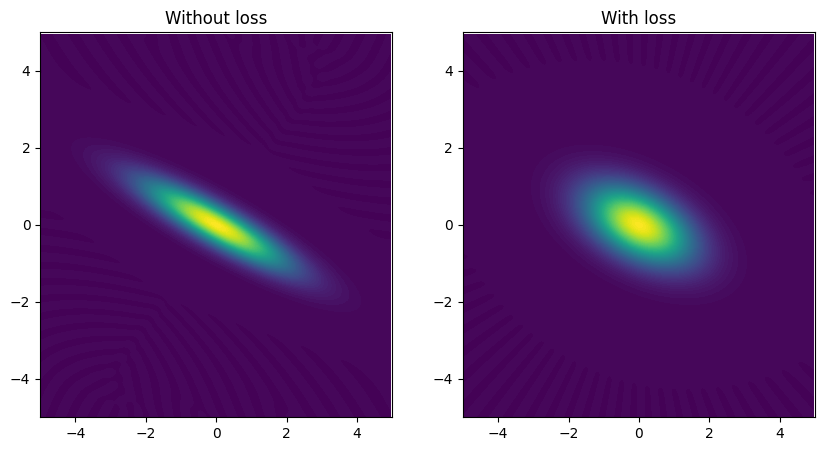
\includegraphics[width=0.4\textwidth]{squeezed_decay_0.5.png}
  \caption{Squeezing by a second-order interaction, compared with the case where the photons are lost to the environment by $\sqrt{\gamma}\hat{a}$. Here, $\alpha$ in $H_{sys}$ is chosen to be $0.2$, and $\gamma$ is chosen to be $0.5$.}
\end{figure}
As can be expected, the Wigner function is transformed into an ellipse, and the lossy distribution displays a level of squeezing much smaller than the non-lossy situation.

Furthermore, to simulate the Wigner function that is not calculable by hand, the Wigner function of a squeezed state generated by a third-order interaction was also simulated in Figure 2.2.
The $H_{sys}$ is given by
\begin{equation}
  \hbar\omega\hat{a}^{\dag}\hat{a}+\hbar\chi^{(3)}\Im\{\underbrace{\alpha^{*} e^{i\omega_{p}t}}_{\text{approx. }\hat{a_{p}}^{\dag}}\hat{a}^{3}\}
\end{equation}
when $\omega_{p}=3\omega$, since the interaction is of third order.
\begin{figure}[htb]
  \centering
  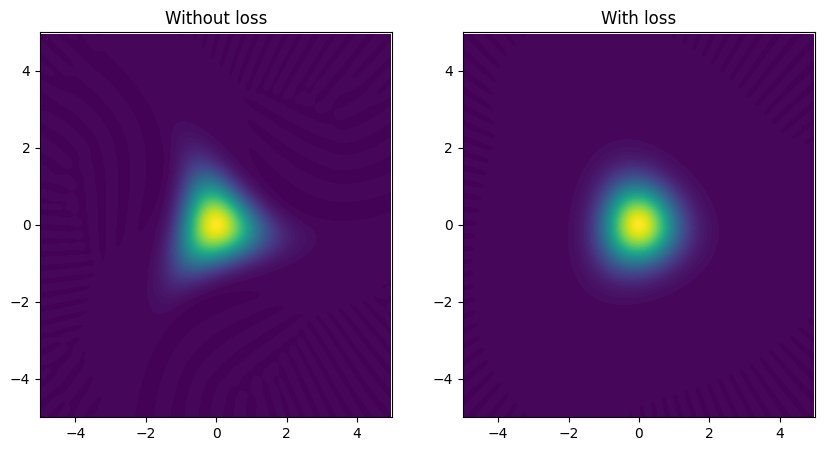
\includegraphics[width=0.4\textwidth]{third_decay_0.5.png}
  \caption{Squeezing by a third-order interaction, compared with the case where the photons are lost to the environment by $\sqrt{\gamma}\hat{a}$. Here, $\alpha$ in $H_{sys}$ is chosen to be $0.2$, and $\gamma$ is chosen to be $0.5$.}
\end{figure}
Here, we can see that the Wigner function evolves to something that looks like an equilateral triangle.
The remaining subsection explains analytically why the Wigner functions evolve to what they are predicted in the above figures.

\section{Analytical Analysis}
\subsection{Second-order Squeezing}
In this section, we show that for \textit{all} initial distributions $W(q, p;0)$, the distribution after $t$ time steps result in $W(q_t,p_t;t)$, with $q_t,p_t$ being related to the original coordinates by a linear transformation.

Recall that the Von Neumann equation for the density operator under second order interaction can be written as:
\[
  \partial_{t}\tilde{\rho}=-\frac{\chi^{(2)}}{2}(\alpha^{*}[a^{2},\tilde{\rho}]-\alpha[(a^{\dag})^{2},\tilde{\rho}])
\]

We want to look at the time evolution of the Wigner quasiprobability distribution.
That is, the Von Neumann equation needs to be converted into a PDE of the Wigner function.
Then the Von Neumann equation turns into
\begin{equation}
  \partial_{t}W=-\frac{\chi^{(2)}}{2}(2\alpha z^{*}\partial_{z}W+2\alpha^{*}z\partial_{z^{*}}W)
\end{equation}

Now we want to evaluate how the Wigner function evolves in time given the distribution at time $0$.
That is, we want to calculate the trajectory $(q(t), p(t))$ that satisfies
\[W(q(t),p(t);t)=W(q(0),p(0);0)\]
for all time $t$.

Differentiating both sides by $t$, we get, by the chain rule,
\[\frac{dz}{dt}\partial_{z}W+\frac{dz^{*}}{dt}\partial_{z^{*}}W+\partial_{t}W=0\]
if we view $W$ as a function of $z=q+ip$ and $z^{*}=q-ip$.

By the time evolution equation, this equation can be summarized into
\[\left(\frac{dz}{dt}-\chi^{(2)}\alpha z^{*}\right)\partial_{z}W+\left(\frac{dz^{*}}{dt}-\chi^{(2)}\alpha^{*} z\right)\partial_{z^{*}}W=0\]

Therefore, if the trajectory $z(t)=q(t)+ip(t)$ satisfies
\[\frac{dz}{dt}=\chi^{(2)}\alpha z^{*}\]
then for any initial condition we can determine the Wigner function at time $t$.

Separating into real and imaginary parts, we have
\[
  \frac{d}{dt}
  \begin{bmatrix}
    q \\
    p
  \end{bmatrix}
  = \chi^{(2)}
  \begin{bmatrix}
    \Re(\alpha) & \Im(\alpha)  \\
    \Im(\alpha) & -\Re(\alpha)
  \end{bmatrix}
  \begin{bmatrix}
    q \\
    p
  \end{bmatrix}
\]
and solving this linear ode results in
\begin{equation}
  \begin{bmatrix}
    q \\
    p
  \end{bmatrix}
  =
  R_{\theta/2}
  \begin{bmatrix}
    e^{\chi^{(2)}rt} & 0                 \\
    0                & e^{-\chi^{(2)}rt}
  \end{bmatrix}
  R_{-\theta/2}
  \begin{bmatrix}
    q(0) \\
    p(0)
  \end{bmatrix}
\end{equation}
when $\alpha=re^{i\theta}$ and $R_{\theta/2}$ is the rotation matrix by $\theta/2$.
Thus, we have shown that for \textit{any} initial distribution the distribution is squeezed by
$e^{\chi^{2}r}$. Such a general statement would've been hard to prove without employing the phase space method.

\subsection{Third-order Squeezing}
In third order squeezing, the Von Neumann equation unfolds to:
\begin{align*}
  i\hbar\partial_{t}\rho & = \hbar\omega[a^{\dag}a, \rho]+\hbar\chi^{(3)}\left[\frac{\alpha^{*}e^{3i\omega t}a^{3}-\alpha e^{-3i\omega t}(a^{\dag})^{3}}{2i}, \rho\right] \\
                         & = \hbar\omega[a^{\dag}a, \rho]+\frac{\hbar\chi^{(3)}}{2i}([\alpha^{*}e^{3i\omega t}a^{3}, \rho]-[\alpha e^{-3i\omega t}(a^{\dag})^{3}, \rho])
\end{align*}

Let $\rho=\exp(-i\omega ta^{\dag}a)\tilde{\rho}\exp(i\omega ta^{\dag}a)$, then
\[\partial_{t}\tilde{\rho}=-\frac{\chi^{(3)}}{2}(\alpha^{*}[a^{3},\tilde{\rho}]-\alpha[(a^{\dag})^{3},\tilde{\rho}])\]
Now, the time evolution of the Wigner function is given by
\begin{equation}
  \partial_{t}W=-\frac{\chi^{(3)}}{2}\left(\alpha^{*}\left(3z^{2}\partial_{z^{*}}W+\frac{1}{4}\partial_{z^{*}}^{3}W\right)+\alpha\left(3(z^{*})^{2}\partial_{z}W+\frac{1}{4}\partial_{z}^{3}W\right)\right)
\end{equation}

Unlike the second-order case, the right hand side cannot be written as a linear combination of $\partial_{z}W$ and $\partial_{z^{*}}W$.
Thus, the time evolution of the function cannot be written simply as the time evolution of the $z(t)$ coordinates.
Instead, to develop an intuition as to why the initial state $\ket{0}$ evolves to an equilateral triangle under third order squeezing, we show how the \textit{rotational symmetry} of the initial distribution is preserved.

We consider the rotated distribution $\tilde{W}(z,z^{*};t)\coloneq W(\omega z, \omega^{-1}z^{*};t)$ when $\omega=\exp(i2\pi/3)$ is the third root of unity.
We will show that $\tilde{W}$ also satisfies the above equation.
Note that
\begin{align}
  \partial_{t}\tilde{W}(z,z^{*};t)     & =\partial_{t}\wigner               \\
  \partial_{z}\tilde{W}(z,z^{*};t)     & =\omega\partial_{z}\wigner         \\
  \partial_{z}^{2}\tilde{W}(z,z^{*};t) & =\omega^{2}\partial_{z}^{2}\wigner \\
  \partial_{z}^{3}\tilde{W}(z,z^{*};t) & =\partial_{z}^{3}\wigner
\end{align}
by the chain rule.

Then we have:
\begin{align*}
  \partial_{t}\tilde{W}(z,z^{*};t) & =\partial_{t}\wigner                                                                                                                                      & (\because (2.6))   \\
                                   & =-\frac{\chi^{(3)}}{2}\left( \alpha^{*}\left( 3(\omega z)^{2}\partial_{z^{*}}\wigner+\frac{1}{4}\partial_{z^{*}}^{3}\wigner\right)\right.                                     \\
                                   & \left.+\alpha\left(3(\omega^{-1}z^{*})^{2}\partial_{z}\wigner+\frac{1}{4}\partial_{z}^{3}\wigner\right)\right)                                            & (\because (2.5))    \\
                                   & =-\frac{\chi^{(3)}}{2}\left( \alpha^{*}\left(3z^{2}\partial_{z^{*}}\tilde{W}(z,z^{*};t)+\frac{1}{2}\partial_{z^{*}}^{3}\tilde{W}(z,z^{*};t)\right)\right.                     \\
                                   & \left.+\alpha\left( 3(z^{*})^{2}\partial_{z}\tilde{W}(z,z^{*};t)+\frac{1}{4}\partial_{z^{*}}^{3}\tilde{W}(z,z^{*};t)\right)\right)                        & (\because (2.7-2.9))
\end{align*}

Thus, we know that
\[\partial_{t}(W-\tilde{W})=-\frac{\chi^{(3)}}{2}\left(\alpha^{*}\left(3z^{2}\partial_{z^{*}}+\frac{1}{4}\partial_{z^{*}}^{3}\right)+\alpha\left(3(z^{*})^{2}\partial_{z}+\frac{1}{4}\partial_{z}^{3}\right)\right)(W-\tilde{W})\]
If we have that for time $0$, $(W-\tilde{W})(q,p;0)=0$, that is, if the probability distribution is symmetric with respect to $120^{\circ}$ rotations, then for the rest of the time, $W-\tilde{W}$ stays $0$. That is, the symmetry is preserved in time.
This can explain why the squeezed vacuum subject to the third order generation process displays a Wigner quasiprobability distribution that is shaped like an equilateral triangle.

In fact, for an arbitrary order $n$, rotational symmetry with respect to $e^{i2\pi/n}$ will be preserved, since the same derivation steps applied above with the chain rule and the binomial formula will still hold.
We can argue that, since at higher $n$ the distribution becomes more and more similar to a circle, the ``most effective'' squeezing happens at second order.
Again, such an observation was possible only because the phase space method was employed.

\chapter{Conclusion}\label{chap:conclusion}

We employed the phase space method, which solves the time evolution of the quasiprobability distribution in the $q$ and $p$ coordinates to analyze the squeezed (vacuum) states of light.
By plotting the distribution at time $t$ using numerical methods, we first developed an intuition of how second- and higher-order interactions squeeze the signal photon.
Next, by actually solving the time evolution equation in terms of the Wigner function, we derived exactly why the second-order squeezing is such an effective method in reducing uncertainty in one phase variable, since it displays exponential squeezing.
Moreover, since for higher order squeezing the rotational symmetry of the initial Gaussian distribution in vacuum state is preserved, we were able to conclude that second-order squeezing is indeed the most practical type of squeezing.
Since quantum operators and wave functions require integration to recover the probabilistic nature of quantum phenomena, the phase space method was most convenient in deriving the above conclusions.
Thus, we conclude that the phase space method is a valid method to analyze quantum phenomena.

\printbibliography

\chapter*{\abstractname} % 초록

이 논문은 압축 상태의 진공 광원의 위그너 함수를 분석하여 수치적으로 어떻게 광원의 진폭과 위상이 압축되는지 보여주고, 수학적으로도 왜 그러한 계산 결과가 나오는지 설명한다. 더 자세하게는, 2계 압축을 통해서는 임의의 초기상태에서 압축이 타원 형태로 일어난다는 것을 보이며, 3차 이상에서는 초기상태가 회전에 대해 대칭이면 그 대칭성이 보존됨을 보인다. 이로써 양자역학적 현상의 분석에 있어 위상 공간 분석 방법이 유용함을 주장한다.
\vfill
주요어 : \paperkeywords

\end{document}
